\title{Cobweb Forests:\\ Kolmogorov--Arnold Networks Without Gradients}
\author{Draft --- working notes}
\date{\today}

\begin{document}
\maketitle

\begin{abstract}
Kolmogorov--Arnold Networks (KANs) place learnable one-variable functions on the edges
of a network and justify the design with the Kolmogorov--Arnold representation theorem.
We ask whether the same theorem can be realised by Cobweb, an incremental
concept-formation system that learns without gradients by sorting each example into a
hierarchy of probabilistic concepts.  A \emph{Cobweb forest} is a network of Cobweb trees
in which the predictions or concept labels of some trees are the inputs of others.  We
prove three things.  \emph{Representation:} one Cobweb tree approximates any continuous
function, and a forest of $4n^2+4n$ two-input trees realises the Kolmogorov--Arnold
representation of any continuous function of $n$ variables; one input per tree is not
enough.  \emph{Learning:} Cobweb never deletes what it has stored, so a learned tree is a
consistent regressor whatever hierarchy it builds, and a learned forest converges to the
forest in which every tree predicts the expectation of its outcome given its inputs.
\emph{Tasks:} without back-propagation a tree can only learn to predict what it will
observe, so the forest must give each tree an observable outcome.  Predicting the final
target works when the parts combine monotonically and fails on interactions such as
$x_1x_2$; categorizing always works but pays for every cell; and no tree can tell its
role from its own data, so the choice must be verified where trees are composed.
Following the KAN paper's experiments, Cobweb forests do not forget in continual
learning and their trees can be plotted like KAN edges, while on smooth targets
gradient-trained KANs and MLPs are far more accurate.  The discrete cores of the
statements are proved in Lean~4 and the rest are checked against the implementation.
\end{abstract}

\tableofcontents

%=====================================================================
\section{Introduction}\label{sec:intro}
%=====================================================================

The Kolmogorov--Arnold (KA) representation theorem
\citep{kolmogorov1957,arnold1957,lorentz1966,sprecher1965} says that every continuous
$f:[0,1]^n\to\R$ can be written as
\begin{equation}\label{eq:ka}
  f(x_1,\dots,x_n)=\sum_{q=0}^{2n}\Phi_q\Bigl(\sum_{p=1}^{n}\varphi_{q,p}(x_p)\Bigr),
\end{equation}
with continuous one-variable functions $\varphi_{q,p}$ (independent of $f$) and $\Phi_q$.
The only operation on several variables is addition.  Kolmogorov--Arnold Networks
\citep{liu2024kan} turn \eqref{eq:ka} into an architecture: learnable splines on the
edges, sums at the nodes, trained by back-propagation.

Cobweb \citep{fisher1987} is a different kind of learner.  It sorts each example down a
tree of probabilistic concepts and, at every node, takes whichever of four operators
(add to the best child, create a child, merge two children, split a child) most
increases \emph{category utility}, the information the concepts carry about the features
\citep{corter1992,maclellan2026rational}.  It learns one example at a time, in closed
form, with no gradient, and it does not forget.  Several systems already wire Cobweb
trees together: Convolutional Cobweb \citep{maclellan2021conv} feeds the concept labels
of patch trees to a classification tree, TRELLIS \citep{singaravadivelan2026trellis}
describes composites by concept identifiers from another tree, and a Cobweb language
model passes each tree's prediction to the trees above it.  We call such a network a
\emph{Cobweb forest} and ask the two questions the KAN paper answers for KANs:
\begin{enumerate}[label=\textbf{Q\arabic*.},leftmargin=*,noitemsep]
\item \emph{Representation.} Can a Cobweb forest represent any continuous function, and
  with how many trees?
\item \emph{Learning.} If every tree learns only by Cobweb's own procedure, does the
  forest learn the function?
\end{enumerate}

\Cref{tab:analogy} lines the three architectures up.  The answer to Q1 is the same as
for KANs: a forest shaped like \eqref{eq:ka} represents $f$ (\cref{sec:repr}).  Q2 has a
twist.  A KAN learns its inner functions from the error of their sum.  A Cobweb tree
receives no error; it can only learn to predict something it will \emph{observe}.  The
values $\Phi_q(\cdot)$ are never observed, so the KA forest cannot be learned as it
stands.  What a learned forest can do depends on what each tree is asked to predict, its
\emph{task}, and \cref{sec:learn} shows which tasks work.

\begin{table}[t]
\centering\small
\begin{tabular}{@{}p{3.1cm}p{3.3cm}p{3.6cm}p{4.6cm}@{}}\toprule
 & MLP & KAN & Cobweb forest\\\midrule
theorem & universal approximation & Kolmogorov--Arnold & Kolmogorov--Arnold (\cref{thm:main-cka})\\
unit & weights, fixed activation & learnable spline on an edge & a Cobweb tree (concept hierarchy)\\
summation & free, at nodes & free, at nodes & a two-input tree\\
what a unit passes & a number & a number & a prediction or a concept label\\
learning & back-propagation & back-propagation & sort and restructure; each tree predicts an observable outcome\\
forgetting & catastrophic & local & none: no stored example is deleted (\cref{thm:main-learn})\\
interpretability & low & plot each edge & plot each tree\\
\bottomrule
\end{tabular}
\caption{MLPs, KANs and Cobweb forests.}
\label{tab:analogy}
\end{table}

\paragraph{Contributions.}
\begin{itemize}[leftmargin=*,noitemsep]
\item One Cobweb tree is a universal approximator with an explicit rate, and a forest of
  $4n^2+4n$ two-input trees realises \eqref{eq:ka}; one input per tree is not enough
  (\cref{sec:repr}).
\item Cobweb never deletes a stored example, so a learned tree is a consistent regressor
  whatever hierarchy category utility builds, and a learned forest converges to the forest
  of conditional expectations its tasks define (\cref{sec:learn}).
\item Which tasks recover $f$: predicting the target, predicting another part of the
  input, or categorizing; and why a tree's task must be chosen where trees are composed
  (\cref{sec:tasks-main}).
\item The KAN paper's experiments repeated for Cobweb forests, plus housing, MNIST and
  text (\cref{sec:exp}); a short cognitive reading (\cref{sec:cog}); and verification by
  Lean proofs, executable checks and an adversarial review (\cref{app:verify}).
\end{itemize}

%=====================================================================
\section{Cobweb trees and forests}\label{sec:forests}
%=====================================================================

\paragraph{A tree as a function.}
A Cobweb tree stores examples $(x,y)$.  Every concept $c$ keeps the count $n_c$ of the
examples below it and their mean $\mu_c=(\mu_{c,x},\mu_{c,y})$ and variance; the leaves
hold the examples themselves.  To predict $y$ at a new $x$, the tree mixes the means of
its leaves, weighting each by how many examples it holds and how well it explains $x$:
\begin{equation}\label{eq:tree}
  \hy(x)=\frac{\sum_{c\text{ leaf}}n_c\,\N(x;\mu_{c,x},h^2)\,\mu_{c,y}}
              {\sum_{c\text{ leaf}}n_c\,\N(x;\mu_{c,x},h^2)},
\end{equation}
where the variance floor $h^2$ plays the role of a bandwidth.  This is the
\emph{count-weighted leaf mixture}.  The implementation also mixes over internal concepts and
offers four weightings; \cref{app:model} defines all of them, and the results below say
which ones they cover.

\paragraph{Forests.}
A \emph{Cobweb forest} is a directed acyclic graph of Cobweb trees with one output tree.
An edge $\sigma\to\tau$ carries one of two \emph{messages} from $\sigma$ into $\tau$'s
examples: its \emph{activation}, the prediction \eqref{eq:tree} of $\sigma$'s outcome,
or its \emph{label}, the identifier of the concept the input sorts to.  A tree may also
read raw coordinates of $x$.  Every tree learns with Cobweb's own procedure on the
examples made of its inputs and its outcome.  In the \emph{online} protocol each tree
first emits its message for a new observation and then learns it, as Cobweb's
predict-then-learn loop does; this keeps a tree's training messages out of sample
(\cref{def:forestlearn}).

%=====================================================================
\section{Representation: a Cobweb--Kolmogorov--Arnold theorem}\label{sec:repr-main}
%=====================================================================

\begin{theorem}[One tree is a universal approximator; \cref{thm:single}]\label{thm:main-single}
Let $g$ be continuous on a compact $K\subset\R^d$.  For every $\varepsilon>0$ there is a
Cobweb tree whose prediction is within $\varepsilon$ of $g$ on all of $K$.  If $g$ is
$L$-Lipschitz, a tree with $G$ leaves achieves error at most
$C_d\,L\,\mathrm{diam}(K)\,G^{-1/d}+C_d\|g\|_\infty G^{-1}$.
\end{theorem}

\emph{Idea.}  Put one leaf at each point of a fine grid, holding $(\gamma,g(\gamma))$.
With a variance floor at the grid spacing, \eqref{eq:tree} is a Gaussian average of
$g$ over the grid points near $x$, and the root's share of the mixture is of order $1/G$.
The same holds for two of the implementation's all-concept weightings, while the other
two keep a fixed bias on such a flat tree (\cref{prop:prior}).

\begin{figure}[t]
\centering
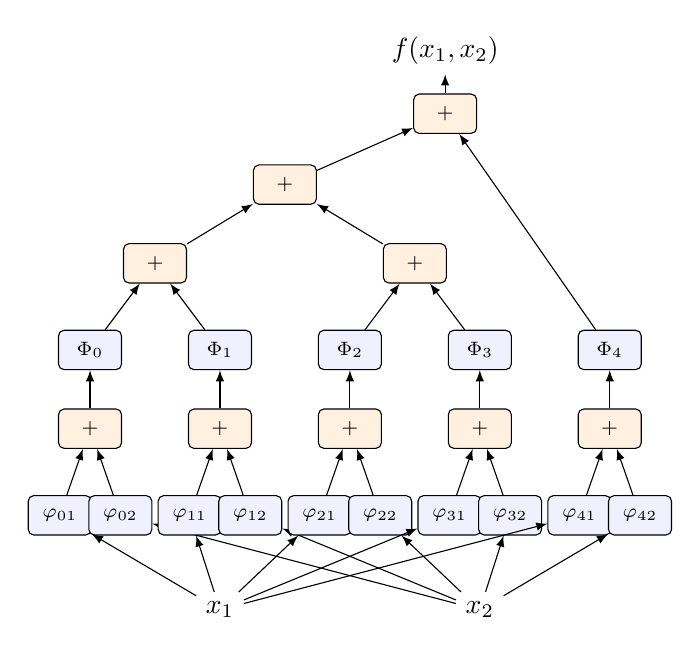
\begin{tikzpicture}[x=1.1cm,y=1cm,
  tree/.style={draw,rounded corners=2pt,minimum width=0.8cm,minimum height=0.5cm,font=\scriptsize,fill=blue!6},
  add/.style={draw,rounded corners=2pt,minimum width=0.8cm,minimum height=0.5cm,font=\scriptsize,fill=orange!12},
  >=latex]
\node (x1) at (1.5,0) {$x_1$};
\node (x2) at (4.5,0) {$x_2$};
\foreach \q/\xx in {0/0,1/1.5,2/3,3/4.5,4/6} {
  \node[tree] (a\q) at (\xx-0.35,1.2) {$\varphi_{\q1}$};
  \node[tree] (b\q) at (\xx+0.35,1.2) {$\varphi_{\q2}$};
  \draw[->] (x1) -- (a\q); \draw[->] (x2) -- (b\q);
  \node[add] (s\q) at (\xx,2.3) {$+$};
  \draw[->] (a\q) -- (s\q); \draw[->] (b\q) -- (s\q);
  \node[tree] (P\q) at (\xx,3.3) {$\Phi_{\q}$};
  \draw[->] (s\q) -- (P\q);
}
\node[add] (o1) at (0.75,4.4) {$+$}; \draw[->] (P0) -- (o1); \draw[->] (P1) -- (o1);
\node[add] (o2) at (3.75,4.4) {$+$}; \draw[->] (P2) -- (o2); \draw[->] (P3) -- (o2);
\node[add] (o3) at (2.25,5.4) {$+$}; \draw[->] (o1) -- (o3); \draw[->] (o2) -- (o3);
\node[add] (o4) at (4.1,6.3) {$+$}; \draw[->] (o3) -- (o4); \draw[->] (P4) -- (o4);
\node (f) at (4.1,7.1) {$f(x_1,x_2)$}; \draw[->] (o4) -- (f);
\end{tikzpicture}
\caption{The Cobweb--Kolmogorov--Arnold forest for $n=2$: every box is a Cobweb tree that
passes its activation.  Blue trees have one input and realise the functions of
\eqref{eq:ka}; orange trees have two inputs and realise the sums.  There are
$4n^2+4n=24$ trees.}
\label{fig:cka}
\end{figure}

\begin{theorem}[Cobweb--Kolmogorov--Arnold; \cref{thm:cka,prop:fanin}]\label{thm:main-cka}
For every continuous $f$ on $[0,1]^n$ and every $\varepsilon>0$ there is a Cobweb forest
of $4n^2+4n$ trees, each with at most two inputs and passing activations, whose output
is within $\varepsilon$ of $f$ (\cref{fig:cka}).  A forest in which every tree has one
input computes a function of a single coordinate, so two inputs per tree are necessary.
\end{theorem}

\emph{Idea.}  Read \eqref{eq:ka} as a graph of one- and two-variable maps:
$n(2n+1)$ inner functions, $(2n+1)(n-1)$ additions for the inner sums, $2n+1$ outer
functions and $2n$ additions for the outer sum.  Replace every map by a tree from
\cref{thm:main-single}.  Errors pass through continuous maps, so choosing each tree's
accuracy backwards from the output keeps the total error below $\varepsilon$
(\cref{lem:dag}).

Three remarks place the theorem.  First, as for KANs, the useful statement assumes
structure: if $f$ is a composition of maps with at most $k$ inputs each, a forest with
$G$ leaves per tree has error of order $G^{-1/k}$, set by the fan-in and not by $n$,
while a single tree pays $G^{-1/n}$ (\cref{rem:rates}).  Second, labels are universal
too: trees that categorize each coordinate and pass their labels to a lookup tree
approximate any $f$, but the lookup tree needs one leaf per cell, $K^n$ in all, because
labels carry no metric (\cref{thm:label}).  Third, merging trees under one common root
does not compose them: the merged tree predicts a mixture of their predictions
(\cref{prop:interweave}).  Composition is what a forest adds to a tree.

%=====================================================================
\section{Learning without gradients}\label{sec:learn-main}
%=====================================================================

\subsection{One tree}

\begin{theorem}[Cobweb never forgets, so a learned tree is consistent;
\cref{lem:leaves,thm:consistency}]\label{thm:main-learn}
None of Cobweb's operators deletes a leaf, and every example ends in exactly one leaf.
Hence, whatever hierarchy category utility builds and in whatever order the examples
arrive, the count-weighted leaf mixture \eqref{eq:tree} of a learned tree equals the
Nadaraya--Watson kernel regression on all examples seen.  If $h\to0$ and $Nh^d\to\infty$,
the learned tree's prediction converges to $\E[Y\mid X=x]$ for every distribution of
$(X,Y)$ with bounded $Y$.
\end{theorem}

The hierarchy plays no role in consistency; it matters for search under a budget, for
the default \textsc{path} weighting, and for the labels a tree passes on
(\cref{rem:structure}).  The weights must count examples: a count-blind mixture averages
distinct stored values instead of samples and fails when examples repeat
(\cref{rem:counts}).

\subsection{A forest learns conditional expectations}

Give every tree $\tau$ a \emph{task}: its inputs $U_\tau$ (raw coordinates and parents'
messages) and an \emph{outcome} $V_\tau$ it will observe.  By \cref{thm:main-learn} each
tree learns $\E[V_\tau\mid U_\tau]$, so the forest has a natural limit, the \emph{ideal
forest}: in topological order, every tree emits $m_\tau=\E[V_\tau\mid U_\tau]$, where
$U_\tau$ is built from the ideal messages of its parents.

\begin{theorem}[A learned forest converges to its ideal forest;
\cref{thm:ideal,cor:iff}]\label{thm:main-forest}
Under regularity conditions (bounded outcomes, inputs with densities, variance floors
that shrink slowly enough, \cref{ass:regular}), the output of a forest learned by Cobweb
converges uniformly to the output $F$ of its ideal forest.  It therefore learns
$f=\E[Y\mid X]$ if and only if $F=f$, i.e.\ if and only if its tasks are
\emph{sufficient}.
\end{theorem}

\Cref{thm:main-forest} separates what Cobweb's learning does from what the tasks
determine.  Every tree learns exactly the conditional expectation of its outcome given
its inputs; whether these compose to $f$ is a property of the tasks alone.

\subsection{What should each tree predict?}\label{sec:tasks-main}

In the KA forest the tree for $\Phi_q$ must hold $\Phi_q(u_q)$, a quantity no one ever
observes; only the sum $f$ is observed (\cref{rem:kaobs}).  A KAN separates the terms of
the sum by back-propagation.  A Cobweb tree can only predict an observable outcome, and
there are three natural kinds:
\emph{funnel} (every tree predicts the target $Y$, as in the Cobweb language model),
\emph{cross-view} (a tree predicts a part of the input it does not see, such as a
neighbouring pixel), and \emph{categorization} (no outcome; the tree passes labels, as in
Convolutional Cobweb).

\begin{proposition}[Which tasks are sufficient; \cref{sec:tasks}]\label{prop:main-tasks}
\leavevmode
\begin{enumerate}[label=(\alph*),leftmargin=*,noitemsep]
\item \emph{Funnel tasks work when the parts combine monotonically}: if
  $Y=\Phi\bigl(\sum_jg_j(X_{B_j})\bigr)+\text{noise}$ with $\Phi$ increasing and
  independent blocks $X_{B_j}$, a forest in which each tree predicts $Y$ is sufficient
  (\cref{prop:suffclass}).
\item \emph{Funnel tasks fail on interactions}: for $Y=X_1X_2$ with symmetric inputs, a
  tree that sees only $X_1$ predicts $\E[Y\mid X_1]=0$, so the funnel forest learns
  nothing (\cref{prop:xy}).
\item \emph{Categorization always works, at a price}: label forests are consistent when
  their cells shrink and stay few compared with the data, which costs a number of cells
  exponential in $n$ (\cref{thm:labelcons}).
\item \emph{Cross-view tasks work when the target lives in what the views share}, as in a
  Gaussian multi-view model (\cref{prop:multiview}).
\end{enumerate}
\end{proposition}

Can a tree find out by itself whether its task is right?  No.

\begin{proposition}[A tree cannot tell its role from its own data;
\cref{thm:locality,cor:parity}]\label{prop:main-local}
Let $X_1,X_2,X_3$ be uniform on $[-1,1]$ and compare $Y=\operatorname{sign}(X_1X_2)$ with
$Y=\operatorname{sign}(X_1X_3)$, observing only $X_1,X_2,Y$.  In the first world $X_2$
is essential; in the second it is irrelevant.  Yet the pair $(X_2,Y)$ has the same
distribution in both, so a tree that sees $X_2$, whatever it predicts, receives the same
data, and every rule based on its own data errs in one of the two worlds.  The same holds
for the parity of any number of signs.
\end{proposition}

The information a tree carries can be synergistic: it exists only together with another
tree's input.  Back-propagation solves this by sending the error of the composition to
every module.  A Cobweb forest must instead decide at the tree that composes the parts.
Choosing among candidate task assignments by the validation error of the output is
consistent: it selects a sufficient assignment with probability tending to one whenever
one is among the candidates (\cref{thm:selection}).  This gives a simple recipe
(\cref{proc:induction}): merge the pairs of inputs whose combination the activations lose
(those with a positive \emph{synergy deficit}, \cref{def:operators}), compose the groups
with two-input trees, and choose each tree's message by validation, always keeping the
single merged tree among the candidates.

%=====================================================================
\section{Experiments}\label{sec:exp}
%=====================================================================

We repeat the KAN paper's experiments \citep{liu2024kan} and add tabular data, images and
text.  Trees use the implementation's defaults (the \textsc{path} weighting over leaves, a
budget of 300 leaves, the online protocol), which lie outside the hypotheses of the
convergence theorems; the experiments test the theorems' predictions rather than
instantiate them.  Errors are test RMSE divided by the standard deviation of $f$, averaged
over three seeds unless stated.  The full setup and further experiments are in
\cref{app:experiments}.  We do not claim that Cobweb forests are competitive regressors:
a Cobweb tree is a nonparametric smoother, and on smooth targets the gradient-trained
MLP and KAN are far more accurate.

\begin{figure}[t]
\centering
\includegraphics[width=\linewidth]{figs/toys.pdf}
\caption{Test RMSE$/\mathrm{sd}(f)$ against $N$ on the KAN paper's toy functions.  Forests
are drawn with their best graph (dotted: the univariate graph of the 4-D target).}
\label{fig:toys}
\end{figure}

\begin{table}[t]
\centering\small
\resizebox{\linewidth}{!}{\input{tables/toys}}
\caption{Toy functions: test RMSE$/\mathrm{sd}(f)$, mean of three seeds.  ``activations''
is the funnel forest; for the 4-D target the forests use the pairs graph (superscript
$u$: univariate graph).}
\label{tab:toys}
\end{table}

\paragraph{Toy functions (\cref{fig:toys,tab:toys}).}
One tree's error falls with $N$ on every target of dimension up to four, as
\cref{thm:main-learn} predicts; on $\sin(\pi x)$ and $\exp(\sin\pi x_1+x_2^2)$ at
$N=16000$ it is 7 to 11 times behind the MLP and 16 to 34 times behind the KAN, and on
$J_0(20x)$ it beats the KAN, whose grid limits it.  On $x_1x_2$ the funnel forest stays at
the error of a constant ($0.99$ to $1.02$), exactly as \cref{prop:main-tasks}(b) predicts,
while label ($0.22$) and hybrid ($0.19$) forests learn.  On the 4-D target
$\exp\bigl(\tfrac12(\sin\pi(x_1^2+x_2^2)+\sin\pi(x_3^2+x_4^2))\bigr)$ the funnel forest over
the two pairs, which is sufficient by \cref{prop:main-tasks}(a), beats the single tree at
small $N$ ($0.46$ against $0.57$ at $N=1000$) and loses at $N=16000$ ($0.33$ against
$0.28$).  On the 100-D target no Cobweb design gets below $0.95$, while the KAN reaches
$0.002$: each univariate tree must estimate a weak signal, and its errors compound
through the levels (\cref{tab:diag100}).

\begin{figure}[t]
\centering
\includegraphics[width=0.9\linewidth]{figs/continual.pdf}
\caption{Continual learning on the KAN paper's five-peak task
\citep[Fig.~3.4]{liu2024kan}; one region per phase (shaded), target in grey.}
\label{fig:continual}
\end{figure}

\paragraph{Continual learning (\cref{fig:continual}).}
\Cref{thm:main-learn} says that a tree never deletes what it has learned.  On the KAN
paper's continual task the tree's error on all data seen so far stays between $0.037$ and
$0.048$ through all five phases; the MLP forgets (its error reaches $10.8$) and the KAN
with a fine grid forgets partly ($0.17$; \cref{tab:continual}).

\begin{figure}[t]
\centering
\includegraphics[width=\linewidth]{figs/interpret.pdf}
\caption{What the trees of a funnel forest learn on $\exp(\sin\pi x_1+x_2^2)$
($N=4000$).  Left and centre: each univariate tree's activation against the exact
$\E[f\mid x_i]$.  Right: the output tree as a function of the two activations.}
\label{fig:interpret}
\end{figure}

\paragraph{Interpretability (\cref{fig:interpret}).}
Like a KAN's edges, a forest's trees can be plotted.  On $\exp(\sin\pi x_1+x_2^2)$ the
univariate trees learn $c_1e^{\sin\pi x_1}$ and $c_2e^{x_2^2}$, the inner functions of the
target up to monotone maps, without gradients.

\paragraph{Choosing tasks.}
The sign worlds of \cref{prop:main-local} behave as predicted (\cref{tab:locality}): the
tree that sees $x_2$ has the same error and the same flat activation in both worlds,
while the composing tree separates them.  Choosing among candidate forests by the
output's validation error never selects the funnel forest on $x_1x_2$ or on the sign
target, and the selected forest is within one percent of the best candidate in every
setting (\cref{tab:selection}).  On Feynman equations the recipe of
\cref{sec:tasks-main} finds the structure of the formula---in $q(E_f+Bv\sin\theta)$ it
groups $B$, $v$ and $\theta$---and it recovers the two blocks of the 4-D target
(\cref{tab:induce}).

\begin{table}[t]
\centering\small
\input{tables/mnist}
\caption{MNIST accuracy (\%, three seeds); one tree per $7\times7$ patch.  ``label'': patch
trees categorize (Convolutional Cobweb); ``cross'': they predict the centre pixels of the
neighbouring patches; ``act'': they predict the class and pass its distribution;
``hybrid'': ``act'' plus labels.}
\label{tab:mnist}
\end{table}

\paragraph{Real data.}
On California housing the funnel forest over natural feature pairs
(longitude--latitude, \dots) beats the single tree at every $N$ ($0.276$ against $0.303$
at $N=16000$, \cref{tab:housing}); MLP and KAN are better still.  On MNIST
(\cref{tab:mnist}) patch trees that predict the class and pass their predicted
distributions reach $94.4\%$, and the hybrid forest $94.9\%$ at $N=20000$, level with the
KAN ($94.5\%$) and below the MLP ($96.8\%$).  Categorizing patch trees reach $86\%$ and
cross-view patch trees $37$--$52\%$: neighbouring pixels do not carry the class, so
\cref{prop:main-tasks}(d) does not apply.  On next-word prediction from four words
(\cref{tab:owt}) generic forests barely improve on one tree; a Cobweb language model
needs its own architecture.

%=====================================================================
\section{A cognitive reading}\label{sec:cog}
%=====================================================================

The three tasks of \cref{sec:tasks-main} are three things a learner can do with what it
perceives: \emph{categorize} it, as in Cobweb's original concept formation;
\emph{predict an outcome} from it, as in associative learning \citep{rescorla1972}; or
\emph{predict another part} of it, as in predictive-processing accounts of perception
\citep{clark2013}.  The theory says when each suffices.  Categories must grow finer with
experience, and so must the trees' acuity, the variance floor $h$; both are forms of
perceptual learning \citep{goldstone1998}.  Outcome prediction compresses a percept to what
matters for the outcome, which works when parts combine monotonically and fails on
interactions.  Perceptual prediction never needs the outcome and works when the outcome
lives in what the views share.  Two further properties have a cognitive flavour.  Cobweb
stores and does not overwrite, which is why a tree does not forget
(\cref{thm:main-learn}).  And \cref{prop:main-local} is a precise form of the
credit-assignment problem \citep{minsky1961}: a module cannot learn its role from what it
alone sees; the decision belongs where the parts are combined and checked against an
observed outcome.

%=====================================================================
\section{Discussion}\label{sec:discussion}
%=====================================================================

\paragraph{Cobweb forest or KAN?}
Use a KAN or an MLP when the target is smooth, the data are plentiful and offline, and
accuracy is what matters: back-propagation fits the inner functions of \eqref{eq:ka}
directly, and no Cobweb design comes close on smooth targets.  A Cobweb forest is the
choice when learning must be incremental, gradient-free and free of forgetting, when the
units should be inspectable concept hierarchies, or when the inputs are symbolic and the
messages should be concepts.

\paragraph{Rules of thumb for composing trees.}
\begin{enumerate}[leftmargin=*,noitemsep]
\item Give every tree an observable outcome, or none (\cref{sec:tasks-main}).
\item Pass activations where parts combine monotonically; merge inputs, or pass labels,
  where they interact (\cref{prop:main-tasks}).
\item Choose a tree's task where its message is used, by the output's validation error,
  and keep the merged tree among the candidates (\cref{prop:main-local}).
\item Keep forests shallow: two inputs per tree suffice in principle, but each level adds
  error that the next level reads as noise (\cref{tab:diag100}).
\item Predict with counts and train predict-then-learn (\cref{rem:counts,def:forestlearn}).
\end{enumerate}

\paragraph{Limitations.}
The convergence theorems assume the split protocol, full expansion, exact matching and
the count-weighted leaf mixture; the experiments use the implementation's defaults.  One
step of \cref{thm:ideal} relies on a standard uniform law for kernel sums, the label-cell
conditions of \cref{thm:labelcons} are not derived from category utility, and the task
recipe is greedy.  The rates are those of nonparametric smoothing.

\appendix
\numberwithin{theorem}{section}
